\documentclass[11pt,letterpaper]{article}
\PassOptionsToPackage{hyphens}{url}
\usepackage[margin=.83in,top=.8in,bottom=.8in,headheight=15pt]{geometry}
\usepackage[T1]{fontenc}
\usepackage{lmodern,amsmath,amssymb,mathtools,bm,booktabs,array,graphicx,tikz}
\usetikzlibrary{arrows.meta,positioning,calc,decorations.pathreplacing,patterns}
\definecolor{ink}{HTML}{17344D}\definecolor{accent}{HTML}{087E8B}\definecolor{pale}{HTML}{EDF5F5}\definecolor{gold}{HTML}{AD6B19}
\providecommand{\dd}{\,\mathrm{d}}\providecommand{\R}{\mathbb{R}}
\providecommand{\E}{\mathbb{E}}\providecommand{\Var}{\operatorname{Var}}
\providecommand{\Cov}{\operatorname{Cov}}\providecommand{\diag}{\operatorname{diag}}
\providecommand{\norm}[1]{\left\lVert#1\right\rVert}
\providecommand{\abs}[1]{\left|#1\right|}
\usepackage{microtype,hyperref,fancyhdr,enumitem,amsthm,sectsty,needspace}
\allsectionsfont{\raggedright}
\hypersetup{colorlinks=true,linkcolor=ink,urlcolor=accent,pdfauthor={Zan Ahmad},pdftitle={Functions, array axes, and planar trajectories / Lecture notes}}
\setlength{\parindent}{0pt}\setlength{\parskip}{6pt}\linespread{1.07}
\setlist{itemsep=3pt,topsep=4pt,leftmargin=*}
\emergencystretch=2em\clubpenalty=10000\widowpenalty=10000
\pagestyle{fancy}\fancyhf{}\fancyhead[L]{\small Scientific Computing in Python / 2027}\fancyhead[R]{\small Lecture 2}
\fancyfoot[L]{\footnotesize Zan Ahmad}\fancyfoot[R]{\footnotesize\thepage}\renewcommand{\headrulewidth}{.3pt}
\newtheorem{proposition}{Proposition}\newtheorem{theorem}{Theorem}\newtheorem{lemma}{Lemma}
\theoremstyle{definition}\newtheorem{definition}{Definition}\newtheorem{example}{Example}
\numberwithin{equation}{section}
\begin{document}
{\small\scshape Scientific Computing in Python / 2027\hfill Lecture 2}\par\medskip
{\raggedright\hyphenpenalty=10000\exhyphenpenalty=10000\LARGE\bfseries\color{ink} Functions, array axes, and planar trajectories\par}\medskip
{\small Lecture notes}\par\bigskip
We now store repeated two-dimensional trajectories in a single array. Its axes identify the trajectory, observation time, and coordinate component. Finite differences produce interval-average velocities. A planar rotation then gives a linear-algebra calculation whose geometric properties can be checked independently of the code.

\section{The axes of a trajectory array}
\hypertarget{note-the-axes-of-a-trajectory-array}{}\label{note:the-axes-of-a-trajectory-array}
{\small \href{slides.html\#frame=the-axes-of-a-trajectory-array\&step=1}{Slides for this section}}\par
Let $p_{ric}$ denote component $c$ of trajectory $r$ at time index $i$. With $R$ trajectories, $T$ observations, and two coordinates, the array shape is $(R,T,2)$. Its shape records a scientific indexing convention. Reshaping or transposing without reference to that convention changes which entries are treated as neighbors.

\[
p\in\R^{R\times T\times2},\qquad p_{ri0}=x_{ri},\quad p_{ri1}=y_{ri}.
\]

Time is axis 1. Component is axis 2.

\subsection*{Indexing an observation}
\begin{minipage}{\linewidth}
\begin{verbatim}
p[r, i, :]       # one two-component position
p[r, :, :]       # one full trajectory
p[:, i, :]       # all positions at one time
\end{verbatim}
\end{minipage}

Each slice retains a different physical question.
\section{Interval-average velocity}
\hypertarget{note-interval-average-velocity}{}\label{note:interval-average-velocity}
{\small \href{slides.html\#frame=interval-average-velocity\&step=1}{Slides for this section}}\par
Subtract adjacent positions along the time axis and divide by the corresponding time increments. The result has one fewer time index because each value belongs to an interval. Strictly increasing finite times are required. A zero interval gives an undefined quotient and a decreasing axis reverses the intended temporal ordering.

\[
v_{ric}=\frac{p_{r,i+1,c}-p_{ric}}{t_{i+1}-t_i}.
\]

The result has shape $(R,T-1,2)$.

\subsection*{Broadcasting the time increments}
\begin{minipage}{\linewidth}
\begin{verbatim}
dp = np.diff(p, axis=1)
dt = np.diff(t)
v = dp / dt[None, :, None]
\end{verbatim}
\end{minipage}

The two singleton axes repeat the same interval durations across trajectories and coordinate components.
\section{Magnitude and threshold indicators}
\hypertarget{note-magnitude-and-threshold-indicators}{}\label{note:magnitude-and-threshold-indicators}
{\small \href{slides.html\#frame=magnitude-and-threshold-indicators\&step=1}{Slides for this section}}\par
The speed associated with an interval-average velocity is its Euclidean magnitude. A threshold indicator is then a Boolean statement about that magnitude. The magnitude of an interval average is generally not the average instantaneous speed if motion changes direction within the interval. The threshold in this example is a numerical teaching parameter.

\[
s_{ri}=\sqrt{v_{ri0}^2+v_{ri1}^2},\qquad I_{ri}=\mathbf1_{\{s_{ri}>s_*\}}.
\]

The strict inequality excludes equality.

\subsection*{A threshold function}
\begin{minipage}{\linewidth}
\begin{verbatim}
def above_threshold(speed, target):
    return speed > target
\end{verbatim}
\end{minipage}

At $s_*=2$, a speed of $2$ does not qualify and $2.01$ does. Missing and nonfinite inputs require a separate policy.
\begin{center}\begin{minipage}{.98\linewidth}\centering
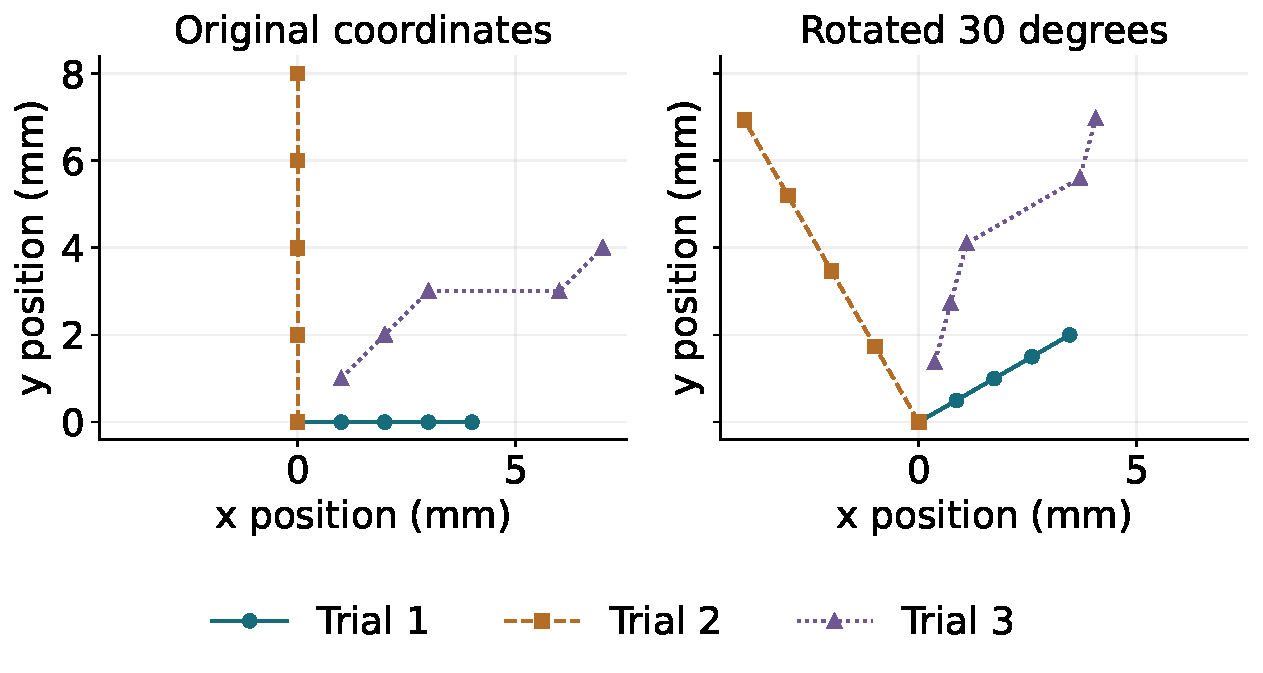
\includegraphics[width=.96\linewidth,height=.57\textheight,keepaspectratio]{trajectory-rotation.pdf}\par\smallskip
{\small A 30-degree plane rotation changes position components while preserving the lengths of corresponding displacement vectors. Lines connect samples only; between-sample motion remains unspecified.}
\end{minipage}\end{center}
\section{A rotation matrix}
\hypertarget{note-a-rotation-matrix}{}\label{note:a-rotation-matrix}
{\small \href{slides.html\#frame=trajectory-rotation-figure\&step=1}{Slides for this section}}\par
A counterclockwise rotation through angle $\theta$ maps column vectors by $p'=Rp$. When vectors occupy rows of an array, the corresponding operation uses $R^{\mathsf T}$ on the right. The sine and cosine functions use radians. At thirty degrees the angle is $\pi/6$.

\[
R(\theta)=\begin{pmatrix}\cos\theta&-\sin\theta\\\sin\theta&\cos\theta\end{pmatrix}.
\]

\[
p'=Rp\quad\text{for columns},\qquad P'=PR^{\mathsf T}\quad\text{for rows}.
\]

\subsection*{Rotation of a basis vector}
At $\theta=\pi/6$,
\[
R\begin{pmatrix}1\\0\end{pmatrix}=\begin{pmatrix}\sqrt3/2\\1/2\end{pmatrix}.
\]

Its length remains one, while its coordinate components change.
\section{Orthogonality and length preservation}
\hypertarget{note-orthogonality-and-length-preservation}{}\label{note:orthogonality-and-length-preservation}
{\small \href{slides.html\#frame=orthogonality-and-length-preservation\&step=1}{Slides for this section}}\par
The columns of a rotation matrix are orthonormal, so $R^{\mathsf T}R=I$. Consequently the squared norm of every displacement is unchanged. Rotation also commutes with subtraction and scalar division, so rotating positions before taking finite differences gives the same velocities as rotating the finite differences.

\[
\|R\Delta p\|_2^2=\Delta p^{\mathsf T}R^{\mathsf T}R\Delta p=\|\Delta p\|_2^2.
\]

Thus every interval speed is unchanged.

\subsection*{Commutation with finite differences}
\[
\frac{Rp_{i+1}-Rp_i}{\Delta t_i}
=R\frac{p_{i+1}-p_i}{\Delta t_i}=Rv_i.
\]

A discrepancy beyond floating-point tolerance suggests an axis or transpose error.
\begin{center}\begin{minipage}{.98\linewidth}\centering
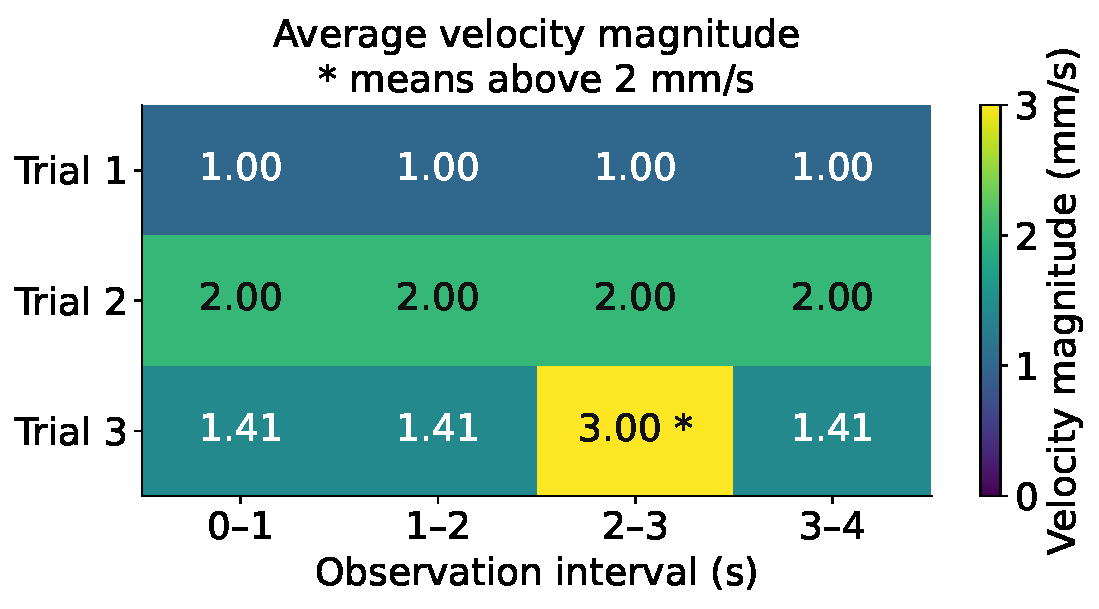
\includegraphics[width=.96\linewidth,height=.57\textheight,keepaspectratio]{speed-shape-map.pdf}\par\smallskip
{\small Each cell is the magnitude of an interval-average velocity in mm/s. The asterisk marks a strict value above 2; it is a display rule rather than a validity or safety classification.}
\end{minipage}\end{center}
\section{Functions with explicit input conditions}
\hypertarget{note-functions-with-explicit-input-conditions}{}\label{note:functions-with-explicit-input-conditions}
{\small \href{slides.html\#frame=functions-with-explicit-input-conditions\&step=1}{Slides for this section}}\par
A trajectory calculation should state its expected axes, units, and admissible times. Validating dimensions before arithmetic produces useful failures near the source of an error. Finite input values can still overflow during a calculation, so the numerical result also requires a finite-value check when supporting arbitrary inputs.

Input conditions include
\[
p\in\R^{R\times T\times2},\quad T\geq2,\quad t_{i+1}>t_i.
\]

Check both the input values and the computed velocities for finiteness.

\subsection*{A geometric test suite}
Translation leaves velocity unchanged. Rotation leaves speed unchanged. Rescaling length by $a$ rescales speed by $|a|$.

These relations test the mathematical operation over many arrays without hard-coding every result.
\bigskip
\section*{Exercises}
\par\noindent\begin{minipage}{\linewidth}
\subsection*{P27-2-1. A reusable interval calculation}
A two-dimensional point moves from (1,-1) mm to (5,2) mm over 2 s. Total: 10 points.

\textbf{a} Calculate the displacement vector, average velocity vector and its magnitude.

\end{minipage}\par\medskip
\textbf{b} Specify one invalid elapsed-time case and the function response. Explain why silently substituting a duration is inappropriate.

\textbf{c} Explain the difference between returning this vector and printing it.

\par\noindent\begin{minipage}{\linewidth}
\subsection*{P27-2-2. Predict every shape}
An array has four trials, seven observation times and two coordinate components. Total: 10 points.

\textbf{a} Give the position, interval-displacement and interval-magnitude shapes.

\end{minipage}\par\medskip
\textbf{b} A duration vector has six entries. Give a broadcast shape that aligns it with intervals and explain both singleton axes.

\textbf{c} Why can checking only the total number of entries miss a scientific error?

\par\noindent\begin{minipage}{\linewidth}
\subsection*{P27-2-3. A rule at its boundary}
A magnitude table contains [1.9,2.0,2.1] mm/s. Total: 10 points.

\textbf{a} State flags for a strict >2 rule, then for a >=\allowbreak{}2 rule.

\end{minipage}\par\medskip
\textbf{b} If all elapsed intervals double with fixed positions, give the new magnitudes and strict flags.

\textbf{c} Does a flag prove an unsafe motion or an invalid sample? Does the magnitude reveal true path speed?

\par\noindent\begin{minipage}{\linewidth}
\subsection*{P27-2-4. Geometry as a check}
Use the 90-degree counterclockwise rotation matrix with rows [0,-1] and [1,0]. Total: 10 points.

\textbf{a} Rotate column vector (2,1) and calculate both old and new lengths.

\end{minipage}\par\medskip
\textbf{b} State the matching operation when points are stored as rows. Why is elementwise multiplication unsuitable?

\textbf{c} Propose two independent checks on a batch rotation.

\section*{References}
\noindent\begin{minipage}{\linewidth}
Original Python Lecture 0. PDF pages 44--45 and 47--49.

\url{https://zanahmad.com/files/scientific-python/Lecture_0__Intro_to_Python.pdf}
\end{minipage}\par\medskip
\noindent\begin{minipage}{\linewidth}
Original Python Lecture 2. PDF pages 30--41.

\url{https://zanahmad.com/files/scientific-python/Lecture_2__Intro_to_Python.pdf}
\end{minipage}\par\medskip
Python source materials: Phillip Kerger (2023). Course adaptation and additional exposition: Zan Ahmad.

\end{document}
